% Block Def
% ---- RC A
\def \rcACenterX{3}
\def \rcACenterY{0}
\def \rcASizeX{2}
\def \rcASizeY{2}

% ---- RC B
\def \rcBCenterX{9.0}
\def \rcBCenterY{0.0}
\def \rcBSizeX{2}
\def \rcBSizeY{2}

% Node Def
\def \nodeRadius{0.2}

% nodeA
\def \nodeACenterX{0}
\def \nodeACenterY{0.0}

% nodeB
\def \nodeBCenterX{6}
\def \nodeBCenterY{0.0}

% nodeC
\def \nodeCCenterX{12}
\def \nodeCCenterY{0.0}

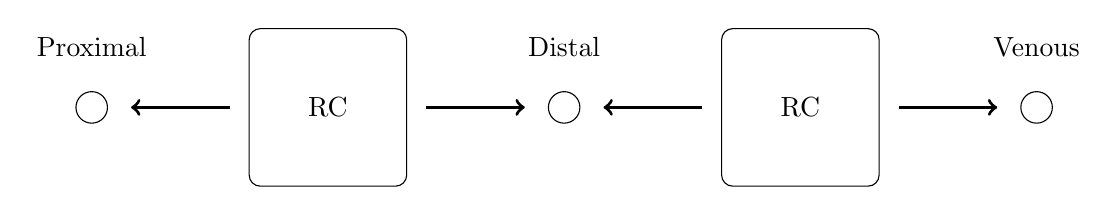
\begin{tikzpicture}
% ---- Nodes circles
% ---- nodeA
\draw (\nodeACenterX, \nodeACenterY) circle [radius = \nodeRadius] node [anchor=south, yshift = 15] {Proximal};
% ---- nodeB
\draw (\nodeBCenterX, \nodeBCenterY) circle [radius = \nodeRadius] node [anchor=south, yshift = 15] {Distal};
% ---- nodeC
\draw (\nodeCCenterX, \nodeCCenterY) circle [radius = \nodeRadius] node [anchor=south, yshift = 15] {Venous};

% ---- RC 1
\draw[rounded corners] (\rcACenterX - \rcASizeX / 2, \rcACenterY - \rcASizeY / 2) rectangle (\rcACenterX + \rcASizeX / 2, \rcACenterY + \rcASizeY / 2) node[pos=.5] {RC};
% ---- RC 2
\draw[rounded corners] (\rcBCenterX - \rcBSizeX / 2, \rcBCenterY - \rcBSizeY / 2) rectangle (\rcBCenterX + \rcBSizeX / 2, \rcBCenterY + \rcBSizeY / 2) node[pos=.5] {RC};

% Flux
\draw [very thick][<-] (\nodeACenterX + 0.5, 0) -- (\rcACenterX - 1.25, 0);
\draw [very thick][->] (\rcACenterX + 1.25, 0) -- (\nodeBCenterX - 0.5, 0);
\draw [very thick][<-] (\nodeBCenterX + 0.5, 0) -- (\rcBCenterX - 1.25, 0);
\draw [very thick][->] (\rcBCenterX + 1.25, 0) -- (\nodeCCenterX - 0.5, 0);
\end{tikzpicture}